\documentclass[tikz]{standalone}
\usepackage[T1]{fontenc}
\usepackage[utf8]{inputenc}
\usepackage{tikz,pgfplots}
\usepackage{grffile}
\pgfplotsset{compat=newest}
\usetikzlibrary{plotmarks,positioning,fit,shapes.geometric,arrows,external,matrix,backgrounds,spy}
\usepgfplotslibrary{patchplots,groupplots,statistics}
\usepackage{siunitx,xcolor,physics}
\usepackage{sfmath}
\renewcommand{\familydefault}{\sfdefault}
\newcommand{\mat}[1]{\mathbf{#1}}

\begin{document}

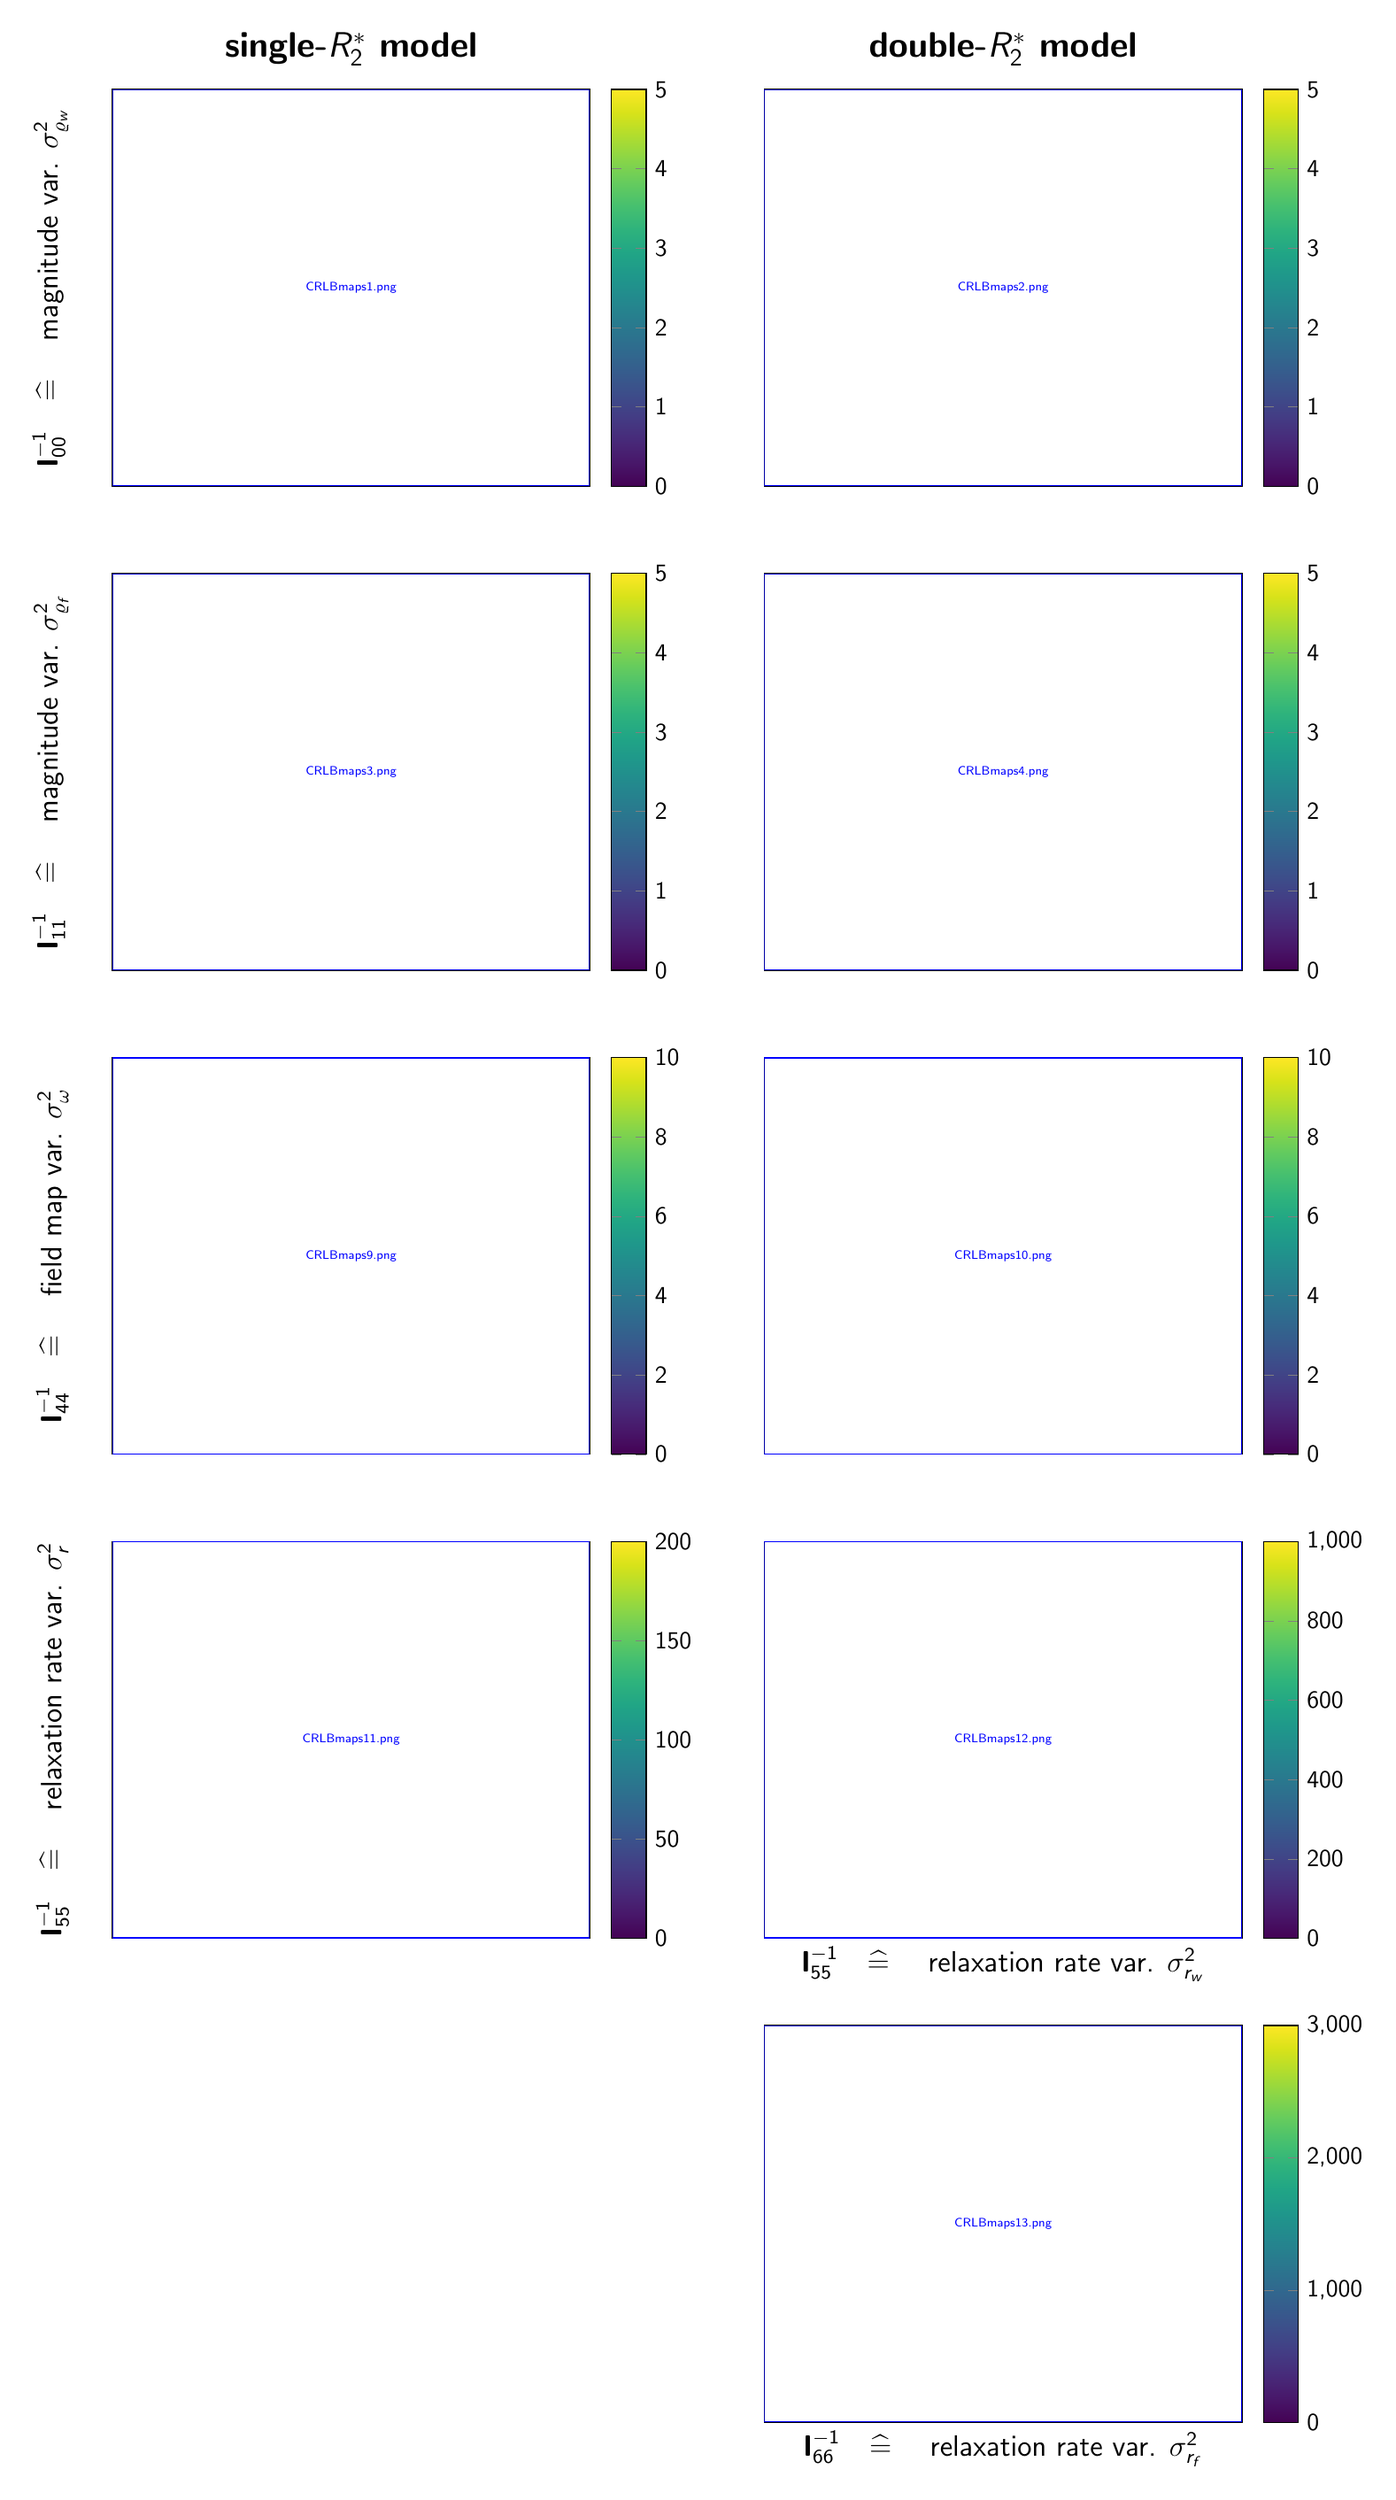
\begin{tikzpicture}
  \pgfplotsset{every axis plot/.append style={line width=4.pt}}
  \pgfplotsset{
    % tick label style = {font=\sansmath\sffamily},
    % every axis label = {font=\sansmath\sffamily},
    % legend style = {font=\sansmath\sffamily},
    title style={font=\large},
    label style = {font=\large}
  }

  \begin{groupplot}[%
    group style={group size=2 by 7,
      horizontal sep=2.5cm,
      vertical sep=1.25cm,
    },
    xmin=-0.5, xmax=223.5,
    ymin=-0.5, ymax=223.5,
    xtick=\empty,
    ytick=\empty,
    colorbar,
    colormap/viridis,
    point meta min=0,
    ylabel style={yshift=0.5cm},
    ]


    \nextgroupplot[
    point meta max=5,
    title={\bf\Large single-\(R_2^{*}\) model},
    ylabel={$\mat{I}^{-1}_{0 0} \quad \widehat{=} \quad$ magnitude var. $\sigma^{2}_{\varrho_w}$},
    ]

    \addplot graphics [includegraphics cmd=\pgfimage,xmin=-0.5, xmax=223.5, ymin=223.5, ymax=-0.5] {CRLBmaps1.png};


    \nextgroupplot[
    point meta max=5,
    title={\bf\Large double-\(R_2^{*}\) model},
    ]

    \addplot graphics [includegraphics cmd=\pgfimage,xmin=-0.5, xmax=223.5, ymin=223.5, ymax=-0.5] {CRLBmaps2.png};


    \nextgroupplot[
    point meta max=5,
    ylabel={$\mat{I}^{-1}_{1 1} \quad \widehat{=} \quad$ magnitude var. $\sigma^{2}_{\varrho_f}$},
    ]

    \addplot graphics [includegraphics cmd=\pgfimage,xmin=-0.5, xmax=223.5, ymin=223.5, ymax=-0.5] {CRLBmaps3.png};


    \nextgroupplot[
    point meta max=5,
    ]

    \addplot graphics [includegraphics cmd=\pgfimage,xmin=-0.5, xmax=223.5, ymin=223.5, ymax=-0.5] {CRLBmaps4.png};


    % \nextgroupplot[
    % point meta max=0.01,
    % ylabel={$\mat{I}^{-1}_{2 2} \quad \widehat{=} \quad$ phase var. $\sigma^{2}_{\phi_w}$},
    % ]

    % \addplot graphics [includegraphics cmd=\pgfimage,xmin=-0.5, xmax=223.5, ymin=223.5, ymax=-0.5] {CRLBmaps5.png};


    % \nextgroupplot[
    % point meta max=0.01,
    % ]

    % \addplot graphics [includegraphics cmd=\pgfimage,xmin=-0.5, xmax=223.5, ymin=223.5, ymax=-0.5] {CRLBmaps6.png};


    % \nextgroupplot[
    % point meta max=0.01,
    % ylabel={$\mat{I}^{-1}_{3 3} \quad \widehat{=} \quad$ phase var. $\sigma^{2}_{\phi_f}$},
    % ]

    % \addplot graphics [includegraphics cmd=\pgfimage,xmin=-0.5, xmax=223.5, ymin=223.5, ymax=-0.5] {CRLBmaps7.png};


    % \nextgroupplot[
    % point meta max=0.01,
    % ]

    % \addplot graphics [includegraphics cmd=\pgfimage,xmin=-0.5, xmax=223.5, ymin=223.5, ymax=-0.5] {CRLBmaps8.png};


    \nextgroupplot[
    point meta max=10,
    ylabel={$\mat{I}^{-1}_{4 4} \quad \widehat{=} \quad$ field map var. $\sigma^{2}_{\omega}$},
    ]

    \addplot graphics [includegraphics cmd=\pgfimage,xmin=-0.5, xmax=223.5, ymin=223.5, ymax=-0.5] {CRLBmaps9.png};


    \nextgroupplot[
    point meta max=10,
    ]

    \addplot graphics [includegraphics cmd=\pgfimage,xmin=-0.5, xmax=223.5, ymin=223.5, ymax=-0.5] {CRLBmaps10.png};


    \nextgroupplot[
    point meta max=200,
    ylabel={$\mat{I}^{-1}_{5 5} \quad \widehat{=} \quad$ relaxation rate var. $\sigma^{2}_{r}$},
    ]

    \addplot graphics [includegraphics cmd=\pgfimage,xmin=-0.5, xmax=223.5, ymin=223.5, ymax=-0.5] {CRLBmaps11.png};


    \nextgroupplot[
    point meta max=1000,
    xlabel={$\mat{I}^{-1}_{5 5} \quad \widehat{=} \quad$ relaxation rate var. $\sigma^{2}_{r_w}$},
    ]

    \addplot graphics [includegraphics cmd=\pgfimage,xmin=-0.5, xmax=223.5, ymin=223.5, ymax=-0.5] {CRLBmaps12.png};


    \nextgroupplot[group/empty plot, colorbar=false]


    \nextgroupplot[
    point meta max=3000,
    xlabel={$\mat{I}^{-1}_{6 6} \quad \widehat{=} \quad$ relaxation rate var. $\sigma^{2}_{r_f}$},
    ]

    \addplot graphics [includegraphics cmd=\pgfimage,xmin=-0.5, xmax=223.5, ymin=223.5, ymax=-0.5] {CRLBmaps13.png};


\end{groupplot}

\end{tikzpicture}


\end{document}